\documentclass[a4paper, 14pt]{extarticle}

% Поля
%--------------------------------------
\usepackage{geometry}
\geometry{a4paper,tmargin=2cm,bmargin=2cm,lmargin=3cm,rmargin=1cm}
%--------------------------------------


%Russian-specific packages
%--------------------------------------
\usepackage[T2A]{fontenc}
\usepackage[utf8]{inputenc} 
\usepackage[english, main=russian]{babel}
%--------------------------------------

\usepackage{textcomp}

% Красная строка
%--------------------------------------
\usepackage{indentfirst}               
%--------------------------------------             


%Graphics
%--------------------------------------
\usepackage{graphicx}
\graphicspath{ {./images/} }
\usepackage{wrapfig}
%--------------------------------------

% Полуторный интервал
%--------------------------------------
\linespread{1.3}                    
%--------------------------------------

%Выравнивание и переносы
%--------------------------------------
% Избавляемся от переполнений
\sloppy
% Запрещаем разрыв страницы после первой строки абзаца
\clubpenalty=10000
% Запрещаем разрыв страницы после последней строки абзаца
\widowpenalty=10000
%--------------------------------------

%Списки
\usepackage{enumitem}

%Подписи
\usepackage{caption} 

%Гиперссылки
\usepackage{hyperref}

\hypersetup {
	unicode=true
}

%Рисунки
%--------------------------------------
\DeclareCaptionLabelSeparator*{emdash}{~--- }
\captionsetup[figure]{labelsep=emdash,font=onehalfspacing,position=bottom}
%--------------------------------------

\usepackage{tempora}
\usepackage{amsmath}
\usepackage{color}
\usepackage{listings}
\lstset{
  belowcaptionskip=1\baselineskip,
  breaklines=true,
  frame=L,
  xleftmargin=\parindent,
  language=Python,
  showstringspaces=false,
  basicstyle=\footnotesize\ttfamily,
  keywordstyle=\bfseries\color{blue},
  commentstyle=\itshape\color{purple},
  identifierstyle=\color{black},
  stringstyle=\color{red},
}

%--------------------------------------
%			НАЧАЛО ДОКУМЕНТА
%--------------------------------------

\begin{document}

%--------------------------------------
%			ТИТУЛЬНЫЙ ЛИСТ
%--------------------------------------
\begin{titlepage}
\thispagestyle{empty}
\newpage


%Шапка титульного листа
%--------------------------------------
\vspace*{-60pt}
\hspace{-65pt}
\begin{minipage}{0.3\textwidth}
\hspace*{-20pt}\centering

\includegraphics[width=\textwidth]{emblem}
\end{minipage}
\begin{minipage}{0.67\textwidth}\small \textbf{
\vspace*{-0.7ex}
\hspace*{-6pt}\centerline{Министерство науки и высшего образования Российской Федерации}
\vspace*{-0.7ex}
\centerline{Федеральное государственное бюджетное образовательное учреждение }
\vspace*{-0.7ex}
\centerline{высшего образования}
\vspace*{-0.7ex}
\centerline{<<Московский государственный технический университет}
\vspace*{-0.7ex}
\centerline{имени Н.Э. Баумана}
\vspace*{-0.7ex}
\centerline{(национальный исследовательский университет)>>}
\vspace*{-0.7ex}
\centerline{(МГТУ им. Н.Э. Баумана)}}
\end{minipage}
%--------------------------------------

%Полосы
%--------------------------------------
\vspace{-25pt}
\hspace{-35pt}\rule{\textwidth}{2.3pt}

\vspace*{-20.3pt}
\hspace{-35pt}\rule{\textwidth}{0.4pt}
%--------------------------------------

\vspace{1.5ex}
\hspace{-35pt} \noindent \small ФАКУЛЬТЕТ\hspace{80pt} <<Информатика и системы управления>>

\vspace*{-16pt}
\hspace{47pt}\rule{0.83\textwidth}{0.4pt}

\vspace{0.5ex}
\hspace{-35pt} \noindent \small КАФЕДРА\hspace{50pt} <<Теоретическая информатика и компьютерные технологии>>

\vspace*{-16pt}
\hspace{30pt}\rule{0.866\textwidth}{0.4pt}
  
\vspace{11em}

\begin{center}
\Large {\bf Лабораторная работа № 1} \\ 
\large {\bf по курсу <<Численные методы линейной алгебры>>} \\ 
\end{center}\normalsize

\vspace{8em}


\begin{flushright}
  {Студент группы ИУ9-71Б Лысенко В. В.\hspace*{15pt} \\
  \vspace{2ex}
  Преподаватель Посевин Д. П.\hspace*{15pt}}
\end{flushright}

\bigskip

\vfill
 

\begin{center}
\textsl{Москва 2024}
\end{center}
\end{titlepage}
%--------------------------------------
%		КОНЕЦ ТИТУЛЬНОГО ЛИСТА
%--------------------------------------

\renewcommand{\ttdefault}{pcr}

\setlength{\tabcolsep}{3pt}
\newpage
\setcounter{page}{2}

\section{Задачи}\label{Sect::task}
\par
\renewcommand{\labelenumii}{\arabic{enumi}.\arabic{enumii}.}
\begin{enumerate} 
    \item Установить Julia
    \item Установить GNUPlot
    \item Настроить Gaston
    \item Установить Jupiter
    \item Настроить вывод графики на базе PyPlot
    \item Настроить Juno
    \item Реализовать вывод трёх произвольных трехмерных графиков
\end{enumerate}

\pagebreak
\section{Практическая реализация}
\par
Для всех трёх фигур структура алгоритма одинакова:
\begin{enumerate} 
    \item Подключить библиотеку, которая предназначена для создания графиков. (Gaston, PyPlot)
    \item Определение диапазона значений для осей (x, y, z для декартовой системы координат и u, v - для полярной).
    \item Построение поверхности с помощью функции surf, принимающей на вход координаты x, y, z.
    \item Отображение графика.
\end{enumerate}
\par
Код для 1-го графика:
\begin{lstlisting}
using Gaston
x = range(-15, stop=15, length=100)
y = range(-15, stop=15, length=100)
surf(x, y, (x,y)->sin.(sqrt.(x.*x+y.*y))./sqrt.(x.*x+y.*y))
\end{lstlisting}

\par
Код для 2-го графика:
\begin{lstlisting}
using Gaston

u = range(0, 3pi, length=100)
v = range(-pi, pi, length=100)
x(u, v) = u .* cos(u) .* (cos(v) + 1)
y(u, v) = u .* sin(u) .* (cos(v) + 1)
z(u, v) = u .* sin(v)

X = [x(ui, vi) for ui in u, vi in v]
Y = [y(ui, vi) for ui in u, vi in v]
Z = [z(ui, vi) for ui in u, vi in v]


surf(X, Y, Z)
\end{lstlisting}

\par
Код для 3-го графика:
\begin{lstlisting}
using PyPlot
x = range(-10, stop=10, length=500)
y = range(-10, stop=10, length=500)
z=@. (x^4)/16+(y/4)'^4-(x'^2*y^2)/8
surf(x, y, z)
PyPlot.display_figs()
\end{lstlisting}
\par
 Cтоит также упомянуть, что символ <<'>> в коде третьей функции отвечает за транспонирование.

\section{Результаты}
1-ый график:
\begin{center}

\includegraphics[scale=0.75]{g1}
\par
\end{center}

2-ой график:
\begin{center}
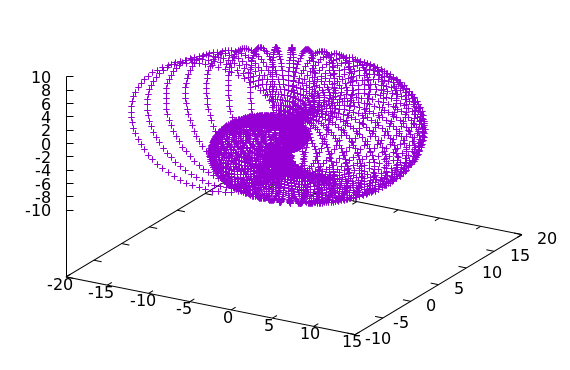
\includegraphics[scale=0.75]{g2}
\par
\end{center}

3-ий график:
\begin{center}
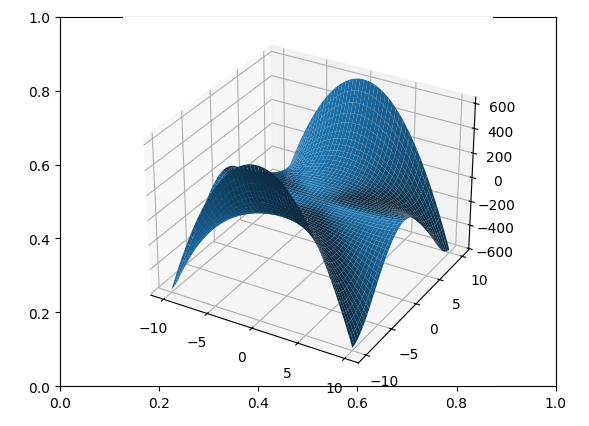
\includegraphics[scale=0.75]{g3}
\end{center}
\section{Выводы}
В данной лабораторной работе были установлены и настроенны инструменты для дальнейшей работы в рамках курса Численных метолов линейной алгебры, а также произведенно знакомство с языком Julia, его возможностями и преимуществами.
\end{document}
